\documentclass[tikz,border=6pt]{standalone}

\usepackage{amsmath}
\usetikzlibrary{3d,arrows.meta,calc}

% =====================================================================
%  3D schematic of the Stern--Gerlach setup
%  Oven -> S1 (slit) -> SG magnet -> S2 (circular aperture) -> Detector
%
%  All coordinates are in mm.  Transverse sizes (x,z) of the magnet are
%  the real ones; the longitudinal distances (y) are schematic and can be
%  changed in the "LAYOUT" block below.
%  Beam propagates along +y, the field gradient is along +z.
% =====================================================================

\begin{document}

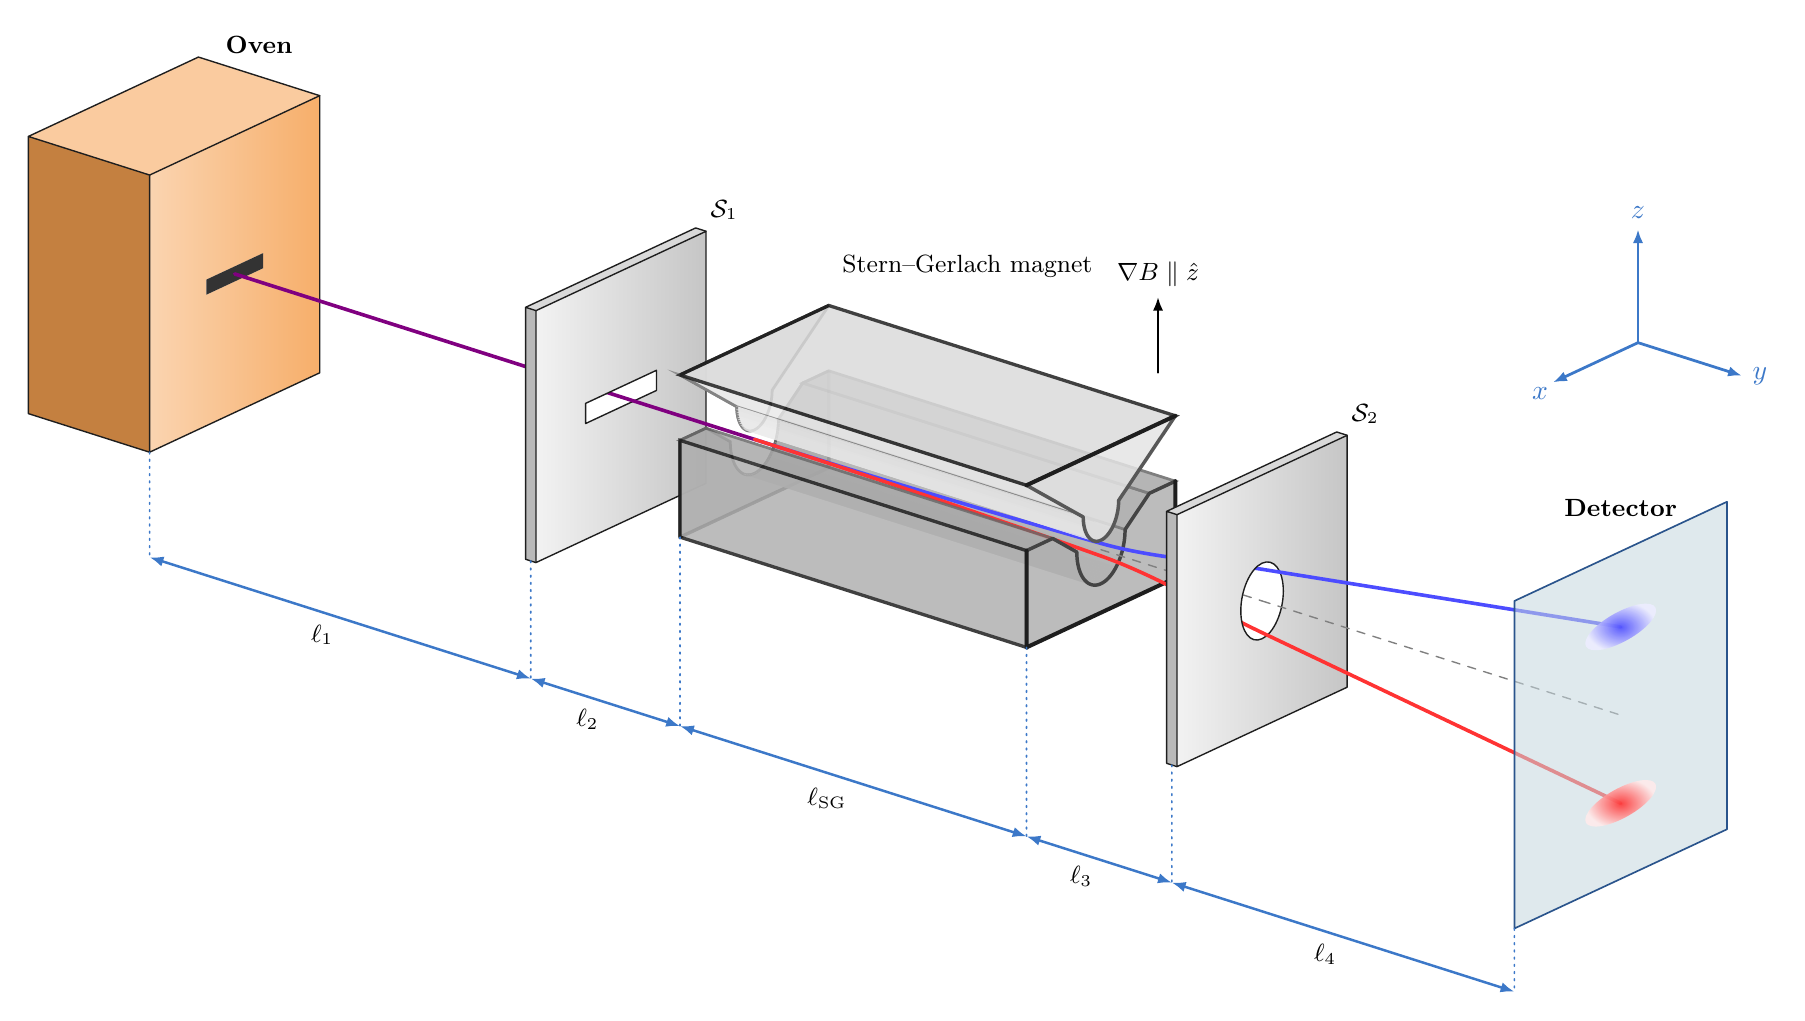
\begin{tikzpicture}[
    % ---- projection: x toward the viewer (left-down), y along the beam, z up
    x={(-0.090cm,-0.042cm)},
    y={( 0.044cm,-0.014cm)},
    z={( 0.000cm, 0.160cm)},
    line join=round, line cap=round,
    dim/.style={{Latex[length=5pt]}-{Latex[length=5pt]}, line width=0.9pt, draw=dimcolor},
    guide/.style={dotted, line width=0.6pt, draw=dimcolor},
]

% ---------------------------------------------------------------------
% Colors
% ---------------------------------------------------------------------
\definecolor{botcolor}{RGB}{150, 150, 150}   % lower pole (trench)
\definecolor{topcolor}{RGB}{195, 195, 195}   % upper pole (arch)
\definecolor{edgecolor}{RGB}{30, 30, 30}
\definecolor{dimcolor}{RGB}{60, 120, 200}
\definecolor{ovencolor}{RGB}{245, 160, 80}
\colorlet{beamcolor}{red!50!blue}
\colorlet{upbeam}{blue!70!white}
\colorlet{downbeam}{red!80!white}

% ---------------------------------------------------------------------
% LAYOUT (y positions, mm) -- schematic, change freely
% ---------------------------------------------------------------------
\pgfmathsetmacro{\lOne}{110}   % oven aperture  -> S1
\pgfmathsetmacro{\lTwo}{40}   % S1             -> magnet entrance
\pgfmathsetmacro{\lSG}{100}   % magnet length
\pgfmathsetmacro{\lThr}{45}   % magnet exit    -> S2
\pgfmathsetmacro{\lFou}{105}   % S2             -> detector

\pgfmathsetmacro{\yOven}{0}
\pgfmathsetmacro{\yOvenBack}{-35}
\pgfmathsetmacro{\ySa}{\yOven+\lOne}
\pgfmathsetmacro{\yMin}{\ySa+\lTwo}
\pgfmathsetmacro{\yMout}{\yMin+\lSG}
\pgfmathsetmacro{\ySb}{\yMout+\lThr}
\pgfmathsetmacro{\yDet}{\ySb+\lFou}

\pgfmathsetmacro{\tp}{1.5}    % half thickness of the plates S1, S2

% Plates / oven / detector transverse half-sizes
\pgfmathsetmacro{\px}{12}  \pgfmathsetmacro{\pz}{10}
\pgfmathsetmacro{\ox}{12}  \pgfmathsetmacro{\oz}{11}
\pgfmathsetmacro{\dx}{15}  \pgfmathsetmacro{\dzz}{13}

% Apertures
\pgfmathsetmacro{\ovenAx}{4.0}  \pgfmathsetmacro{\ovenAz}{0.6}  % oven slit half-sizes
\pgfmathsetmacro{\saAx}{5.0}    \pgfmathsetmacro{\saAz}{0.8}    % S1 slit half-sizes
\pgfmathsetmacro{\sbR}{3.0}                                     % S2 radius

% ---------------------------------------------------------------------
% Magnet cross-section (identical to the stand-alone magnet figure)
% ---------------------------------------------------------------------
\pgfmathsetmacro{\xmin}{-10.5}
\pgfmathsetmacro{\xmax}{ 10.5}
\pgfmathsetmacro{\zmin}{-5.0}
\pgfmathsetmacro{\aa}{2.5}
\pgfmathsetmacro{\zc}{1.3*\aa}
\pgfmathsetmacro{\redge}{1.0*\aa}
\pgfmathsetmacro{\rtrench}{1.362*\aa}
\pgfmathsetmacro{\rtrenchc}{(1.3 - 1.018)*\aa}
\pgfmathsetmacro{\lw}{1.58*\aa}
\pgfmathsetmacro{\phi}{30}
\pgfmathsetmacro{\m}{tan(\phi)}
\pgfmathsetmacro{\xledge}{\rtrench + \lw*cos(\phi)}
\pgfmathsetmacro{\zledge}{\rtrenchc + \lw*sin(\phi)}
\pgfmathsetmacro{\zup}{\zc + \m*(\xmax - \redge)}

\def\poleFaceLW{1.25pt}            % profile width on the face toward S2
\def\opTop{0.85}                  % opacity of the upper pole (1 = solid)
\def\opBot{0.85}                  % opacity of the lower pole (1 = solid)

% ---------------------------------------------------------------------
% Shading of the (opaque) magnet
%   brightness = \shMin + (100-\shMin) * max(0, n.L)   [% of base color]
%   L = light direction (unit vector), n = outward face normal
% ---------------------------------------------------------------------
\def\Lx{0.15}  \def\Ly{0.15}  \def\Lz{0.40}
\def\shMin{120}
% View direction (toward the viewer), derived from the x,y,z vectors
% of the tikzpicture:  V = (y1, -x1, (y2*x1 - x2*y1)/z2).  Faces with
% n.V < 0 point away from the viewer and are not drawn.
\def\Vx{0.044}  \def\Vy{0.090}  \def\Vz{0.0194}

% ---------------------------------------------------------------------
% Beam trajectories (deflection exaggerated for clarity)
% ---------------------------------------------------------------------
\pgfmathsetmacro{\dzm}{0.5}   % |z| at magnet exit
\pgfmathsetmacro{\zdet}{7.0}  % |z| at detector
\pgfmathsetmacro{\kk}{(\zdet-\dzm)/(\yDet-\yMout)}
\pgfmathsetmacro{\zSb}{\dzm+\kk*(\ySb+\tp-\yMout)}

% Dimension line: runs along y at (x = \xdim, z = \zdim), below all parts.
% Every guide drops straight down (along -z) from the bottom edge of its
% part at x = \xdim, so all guides are parallel and start on the part.
% \xdim must lie within the x-range of every part (|x| <= 10.5 mm).
\pgfmathsetmacro{\xdim}{\xmax}
\pgfmathsetmacro{\zdim}{-20}

% =====================================================================
% Helper macros
% =====================================================================

% Magnet cross-section outlines at a given y  (#1 = y)
\newcommand{\topProfile}[1]{%
    (\xmin,#1,\zup) -- (\xmax,#1,\zup) -- (\redge,#1,\zc)
    -- plot[domain=360:180, samples=60, variable=\ang]
        ({\redge*cos(\ang)},#1,{\zc+\redge*sin(\ang)})
    -- cycle}
\newcommand{\botProfile}[1]{%
    (\xmin,#1,\zmin) -- (\xmax,#1,\zmin) -- (\xmax,#1,\zledge)
    -- (\xledge,#1,\zledge) -- (\rtrench,#1,\rtrenchc)
    -- plot[domain=0:180, samples=60, variable=\ang]
        ({\rtrench*cos(\ang)},#1,{\rtrenchc-\rtrench*sin(\ang)})
    -- (-\xledge,#1,\zledge) -- (\xmin,#1,\zledge) -- cycle}

% Inner (pole-face) profile lines of one end face  (#1 = y)
% Optional #1 = line width of the pole-face profile (default 1.0pt);
% the outer outline is always drawn 0.2pt thicker.
\newcommand{\poleLines}[2][1.0pt]{%
    \draw[topcolor!45!black, line width=#1]
        (\xmax,#2,\zup) -- (\redge,#2,\zc)
        -- plot[domain=360:180, samples=60, variable=\ang]
            ({\redge*cos(\ang)},#2,{\zc+\redge*sin(\ang)})
        -- (\xmin,#2,\zup);
    \draw[botcolor!45!black, line width=#1]
        (\xmax,#2,\zledge) -- (\xledge,#2,\zledge) -- (\rtrench,#2,\rtrenchc)
        -- plot[domain=0:180, samples=60, variable=\ang]
            ({\rtrench*cos(\ang)},#2,{\rtrenchc-\rtrench*sin(\ang)})
        -- (-\xledge,#2,\zledge) -- (\xmin,#2,\zledge);
    \draw[edgecolor, line width={#1+0.2pt}]
        (\xmin,#2,\zup) -- (\xmax,#2,\zup)
        (\xmin,#2,\zmin) -- (\xmax,#2,\zmin)
        (\xmin,#2,\zmin) -- (\xmin,#2,\zledge)
        (\xmax,#2,\zmin) -- (\xmax,#2,\zledge);
}

% Brightness \sh for a face with outward normal (#1,#2,#3)
\newcommand{\setshade}[3]{%
    \pgfmathtruncatemacro{\sh}{\shMin+(100-\shMin)*max(0,(#1)*\Lx+(#2)*\Ly+(#3)*\Lz)}}

% Flat magnet surface: #1 = base color, #2 = normal "nx,ny,nz",
% #3 = edge style, #4 = polygon
\newcommand{\magface}[4]{%
    \setshade#2
    \filldraw[fill=#1!\sh!black, #3] #4;}

% Thin plate centred at y = #1 ; #2 = aperture path in the xz canvas
\newcommand{\plate}[2]{%
    % side (+x) and top (+z) faces
    \fill[gray!55] (\px,#1-\tp,-\pz) -- (\px,#1+\tp,-\pz)
                -- (\px,#1+\tp,\pz) -- (\px,#1-\tp,\pz) -- cycle;
    \fill[gray!30] (-\px,#1-\tp,\pz) -- (\px,#1-\tp,\pz)
                -- (\px,#1+\tp,\pz) -- (-\px,#1+\tp,\pz) -- cycle;
    % downstream face with the aperture cut out
    \begin{scope}[canvas is xz plane at y=#1+\tp]
        \shade[left color=gray!10, right color=gray!45, even odd rule]
            (-\px,-\pz) rectangle (\px,\pz) #2;
        \draw[edgecolor, line width=0.5pt] (-\px,-\pz) rectangle (\px,\pz);
        \draw[edgecolor, line width=0.5pt] #2;
    \end{scope}
    \draw[edgecolor, line width=0.5pt]
        (\px,#1+\tp,-\pz) -- (\px,#1-\tp,-\pz) -- (\px,#1-\tp,\pz)
        -- (-\px,#1-\tp,\pz) -- (-\px,#1+\tp,\pz)
        (\px,#1-\tp,\pz) -- (\px,#1+\tp,\pz);
}

% =====================================================================
% 1) OVEN
% =====================================================================
\fill[ovencolor!80!black]
    (\ox,\yOvenBack,-\oz) -- (\ox,\yOven,-\oz) -- (\ox,\yOven,\oz) -- (\ox,\yOvenBack,\oz) -- cycle;
\fill[ovencolor!55]
    (-\ox,\yOvenBack,\oz) -- (\ox,\yOvenBack,\oz) -- (\ox,\yOven,\oz) -- (-\ox,\yOven,\oz) -- cycle;
\begin{scope}[canvas is xz plane at y=\yOven]
    \shade[left color=ovencolor!45, right color=ovencolor!85, even odd rule]
        (-\ox,-\oz) rectangle (\ox,\oz)
        (-\ovenAx,-\ovenAz) rectangle (\ovenAx,\ovenAz);
    \fill[black!80] (-\ovenAx,-\ovenAz) rectangle (\ovenAx,\ovenAz);
    \draw[edgecolor, line width=0.5pt] (-\ox,-\oz) rectangle (\ox,\oz);
\end{scope}
\draw[edgecolor, line width=0.5pt]
    (\ox,\yOven,-\oz) -- (\ox,\yOvenBack,-\oz) -- (\ox,\yOvenBack,\oz)
    -- (-\ox,\yOvenBack,\oz) -- (-\ox,\yOven,\oz)
    (\ox,\yOvenBack,\oz) -- (\ox,\yOven,\oz);

% beam: oven -> S1
\draw[beamcolor, line width=1.3pt] (0,\yOven,0) -- (0,\ySa+\tp,0);

% =====================================================================
% 2) PLATE S1  (rectangular slit)
% =====================================================================
\plate{\ySa}{(-\saAx,-\saAz) rectangle (\saAx,\saAz)}

% =====================================================================
% 3) Beam before the magnet
% =====================================================================
\draw[beamcolor, line width=1.3pt] (0,\ySa+\tp,0) -- (0,\yMin,0);

% =====================================================================
% 4) STERN--GERLACH MAGNET (opaque, shaded extrusion of the cross-section)
%    Painter's order: surfaces behind the beam -> beam -> surfaces in
%    front of the beam -> end face toward S2.
% =====================================================================
\tikzset{
    botedge/.style={draw=botcolor!70!black, line width=1.0pt},
    topedge/.style={draw=topcolor!70!black, line width=1.0pt},
    outedge/.style={draw=edgecolor, line width=1.2pt},
}

% --- end face toward S1: it faces away from the viewer, so it is drawn
%     first (behind everything). It only shows through transparent poles.
\setshade{0}{-1}{0}
\begin{scope}[transparency group, opacity=\opBot]
    \fill[botcolor!\sh!black] \botProfile{\yMin};
\end{scope}
\begin{scope}[transparency group, opacity=\opTop]
    \fill[topcolor!\sh!black] \topProfile{\yMin};
\end{scope}
\pgfmathsetmacro{\opEnd}{min(\opTop,\opBot)}
\begin{scope}[transparency group, opacity=\opEnd]
    \poleLines{\yMin}
\end{scope}

% Each block below is a transparency group: it is drawn opaque and then
% faded as a whole with \opBot / \opTop, so overlapping strips and edges
% inside a pole do not produce darker seams.

\begin{scope}[transparency group, opacity=\opBot]   % ---- lower pole, behind beam
% --- trench (bottom pole groove): only strips facing the viewer
\foreach \i in {0,1,...,35}{
    \pgfmathsetmacro{\angA}{\i*5}
    \pgfmathsetmacro{\angB}{(\i+1)*5}
    \pgfmathsetmacro{\nx}{-cos((\i+0.5)*5)}
    \pgfmathsetmacro{\nz}{ sin((\i+0.5)*5)}
    \pgfmathsetmacro{\vis}{\nx*\Vx+\nz*\Vz}
    \ifdim\vis pt>0pt
        \setshade{\nx}{0}{\nz}
        \filldraw[botcolor!\sh!black, line width=0.3pt]
            ({\rtrench*cos(\angA)},\yMin,{\rtrenchc-\rtrench*sin(\angA)})
            -- ({\rtrench*cos(\angA)},\yMout,{\rtrenchc-\rtrench*sin(\angA)})
            -- ({\rtrench*cos(\angB)},\yMout,{\rtrenchc-\rtrench*sin(\angB)})
            -- ({\rtrench*cos(\angB)},\yMin,{\rtrenchc-\rtrench*sin(\angB)}) -- cycle;
        \draw[botedge]
            ({\rtrench*cos(\angA)},\yMin,{\rtrenchc-\rtrench*sin(\angA)})
            -- ({\rtrench*cos(\angB)},\yMin,{\rtrenchc-\rtrench*sin(\angB)});
    \fi
}

% --- far (-x) slanted wall and ledge of the bottom pole
\magface{botcolor}{{0.5}{0}{0.866}}{botedge}
    {(-\rtrench,\yMin,\rtrenchc) -- (-\xledge,\yMin,\zledge)
     -- (-\xledge,\yMout,\zledge) -- (-\rtrench,\yMout,\rtrenchc) -- cycle}
\magface{botcolor}{{0}{0}{1}}{botedge}
    {(\xmin,\yMin,\zledge) -- (-\xledge,\yMin,\zledge)
     -- (-\xledge,\yMout,\zledge) -- (\xmin,\yMout,\zledge) -- cycle}
\end{scope}

% --- beam inside the magnet (mostly hidden by the poles)
\draw[upbeam, line width=1.3pt]
    plot[domain=\yMin:\yMout, samples=40, variable=\t]
        (0,\t,{\dzm*((\t-\yMin)/\lSG)^2});
\draw[downbeam, line width=1.3pt]
    plot[domain=\yMin:\yMout, samples=40, variable=\t]
        (0,\t,{-\dzm*((\t-\yMin)/\lSG)^2});

\begin{scope}[transparency group, opacity=\opBot]   % ---- lower pole, in front of beam
% --- near (+x) ledge and outer side of the bottom pole
\magface{botcolor}{{0}{0}{1}}{botedge}
    {(\xledge,\yMin,\zledge) -- (\xmax,\yMin,\zledge)
     -- (\xmax,\yMout,\zledge) -- (\xledge,\yMout,\zledge) -- cycle}
\magface{botcolor}{{1}{0}{0}}{outedge}
    {(\xmax,\yMin,\zmin) -- (\xmax,\yMout,\zmin)
     -- (\xmax,\yMout,\zledge) -- (\xmax,\yMin,\zledge) -- cycle}
\end{scope}

\begin{scope}[transparency group, opacity=\opTop]   % ---- upper pole
% --- top pole: near (+x) flank underside
\magface{topcolor}{{0.5}{0}{-0.866}}{topedge}
    {(\redge,\yMin,\zc) -- (\xmax,\yMin,\zup)
     -- (\xmax,\yMout,\zup) -- (\redge,\yMout,\zc) -- cycle}

% --- top pole: rounded tip, only strips facing the viewer
\foreach \i in {0,1,...,35}{
    \pgfmathsetmacro{\angA}{180+\i*5}
    \pgfmathsetmacro{\angB}{180+(\i+1)*5}
    \pgfmathsetmacro{\nx}{cos(180+(\i+0.5)*5)}
    \pgfmathsetmacro{\nz}{sin(180+(\i+0.5)*5)}
    \pgfmathsetmacro{\vis}{\nx*\Vx+\nz*\Vz}
    \ifdim\vis pt>0pt
        \setshade{\nx}{0}{\nz}
        \filldraw[topcolor!\sh!black, line width=0.3pt]
            ({\redge*cos(\angA)},\yMin,{\zc+\redge*sin(\angA)})
            -- ({\redge*cos(\angA)},\yMout,{\zc+\redge*sin(\angA)})
            -- ({\redge*cos(\angB)},\yMout,{\zc+\redge*sin(\angB)})
            -- ({\redge*cos(\angB)},\yMin,{\zc+\redge*sin(\angB)}) -- cycle;
        \draw[topedge]
            ({\redge*cos(\angA)},\yMin,{\zc+\redge*sin(\angA)})
            -- ({\redge*cos(\angB)},\yMin,{\zc+\redge*sin(\angB)});
    \fi
}

% --- top pole: flat top
\magface{topcolor}{{0}{0}{1}}{outedge}
    {(\xmin,\yMin,\zup) -- (\xmax,\yMin,\zup)
     -- (\xmax,\yMout,\zup) -- (\xmin,\yMout,\zup) -- cycle}
\end{scope}

% --- end face toward S2 (drawn last, on top of everything)
\setshade{0}{1}{0}
\fill[topcolor!\sh!black, fill opacity=\opTop] \topProfile{\yMout};
\fill[botcolor!\sh!black, fill opacity=\opBot] \botProfile{\yMout};
\poleLines[\poleFaceLW]{\yMout}   % outline kept fully opaque

% --- beams from the magnet exit to S2
\draw[gray, dashed, line width=0.5pt] (0,\yMout,0) -- (0,\ySb+\tp,0);
% (smooth join between the in-magnet parabola and the straight flight)
\pgfmathsetmacro{\hh}{(\ySb+\tp-\yMout)/3}
\pgfmathsetmacro{\sx}{2*\dzm/\lSG}   % slope at the magnet exit
\draw[upbeam, line width=1.3pt] (0,\yMout,\dzm)
    .. controls (0,\yMout+\hh,{\dzm+\sx*\hh}) and (0,\ySb+\tp-\hh,{\zSb-\kk*\hh})
    .. (0,\ySb+\tp,\zSb);
\draw[downbeam, line width=1.3pt] (0,\yMout,-\dzm)
    .. controls (0,\yMout+\hh,{-\dzm-\sx*\hh}) and (0,\ySb+\tp-\hh,{-\zSb+\kk*\hh})
    .. (0,\ySb+\tp,-\zSb);

% gradient direction
\draw[-{Latex[length=5pt]}, line width=0.9pt]
    (-\xmax,\yMin+0.95*\lSG,\zup+3) -- ++(0,0,6)
    node[above, font=\small] {$\nabla B \parallel \hat{z}$};

% =====================================================================
% 5) PLATE S2  (circular aperture)
% =====================================================================
\plate{\ySb}{(0,0) circle (\sbR)}

% beams: S2 -> detector
\draw[gray, dashed, line width=0.5pt] (0,\ySb+\tp,0) -- (0,\yDet,0);
\draw[upbeam,   line width=1.3pt] (0,\ySb+\tp, \zSb) -- (0,\yDet, \zdet);
\draw[downbeam, line width=1.3pt] (0,\ySb+\tp,-\zSb) -- (0,\yDet,-\zdet);

% =====================================================================
% 6) DETECTOR (semi-transparent screen) + SG pattern
% =====================================================================
\begin{scope}[canvas is xz plane at y=\yDet]
    \fill[cyan!30!gray!40, fill opacity=0.55] (-\dx,-\dzz) rectangle (\dx,\dzz);
    \draw[dimcolor!70!black, line width=0.6pt] (-\dx,-\dzz) rectangle (\dx,\dzz);
    \shade[inner color=upbeam,   outer color=upbeam!10,   opacity=0.9] (0, \zdet) ellipse (5 and 1.3);
    \shade[inner color=downbeam, outer color=downbeam!10, opacity=0.9] (0,-\zdet) ellipse (5 and 1.3);
\end{scope}

% =====================================================================
% 7) DIMENSIONS
% =====================================================================
% Guides start exactly at the near bottom corner of each part and drop
% vertically (on the page) until they meet the dimension line, so they
% stay parallel whatever the part sizes and distances are.
\coordinate (dimA) at (\xdim,\yOven,\zdim);   % two points defining
\coordinate (dimB) at (\xdim,\yDet,\zdim);    % the dimension line
% #1 = name of the foot point on the dimension line, #2 = start corner
\newcommand{\dimguide}[2]{%
    \coordinate (c#1) at #2;
    \coordinate (d#1) at ($(c#1)+(0,-1cm)$);
    \coordinate (#1) at (intersection of c#1--d#1 and dimA--dimB);
    \draw[guide] (c#1) -- (#1);}
\dimguide{g0}{(\ox,\yOven,-\oz)}      % oven aperture face
\dimguide{g1}{(\px,\ySa,-\pz)}        % S1 (centre of the plate)
\dimguide{g2}{(\xmax,\yMin,\zmin)}    % magnet entrance
\dimguide{g3}{(\xmax,\yMout,\zmin)}   % magnet exit
\dimguide{g4}{(\px,\ySb,-\pz)}        % S2 (centre of the plate)
\dimguide{g5}{(\dx,\yDet,-\dzz)}      % detector

\foreach \a/\b/\lab in {g0/g1/{\ell_1}, g1/g2/{\ell_2}, g2/g3/{\ell_{\mathrm{SG}}},
                        g3/g4/{\ell_3}, g4/g5/{\ell_4}}{
    \draw[dim] (\a) -- (\b);
    \node[below left=-1pt, font=\small] at ($(\a)!0.5!(\b)$) {$\lab$};
}

% =====================================================================
% 8) LABELS
% =====================================================================
\node[font=\bfseries\small, anchor=south] at (-\ox,{0.5*(\yOven+\yOvenBack)},\oz+1) {Oven};
\node[font=\small, anchor=south west]     at (-\px,\ySa,\pz) {$\mathcal{S}_1$};
\node[font=\small, anchor=south] at (-\xmax,\yMin+0.40*\lSG,\zup+5)
    {Stern--Gerlach magnet};
\node[font=\small, anchor=south west]     at (-\px,\ySb,\pz) {$\mathcal{S}_2$};
\node[font=\bfseries\small, anchor=south] at (0,\yDet,\dzz+2) {Detector};

% =====================================================================
% 9) COORDINATE TRIAD
% =====================================================================
\begin{scope}[shift={(0,\yDet+5,30)}]
    \draw[-{Latex[length=5pt]}, line width=1.0pt, dimcolor] (0,0,0) -- (12,0,0) node[below left=-2pt] {$x$};
    \draw[-{Latex[length=5pt]}, line width=1.0pt, dimcolor] (0,0,0) -- (0,30,0) node[right]            {$y$};
    \draw[-{Latex[length=5pt]}, line width=1.0pt, dimcolor] (0,0,0) -- (0,0,9)  node[above]            {$z$};
\end{scope}

\end{tikzpicture}

\end{document}
